\documentclass[12pt, letterpaper]{article}
\usepackage{graphicx}
\usepackage[T1]{fontenc}
\usepackage[polish]{babel}
\usepackage[utf8]{inputenc}

\graphicspath{{images/}}

%--------------------------------------------------------------------------------------------------
%       TITLE SECTION
%--------------------------------------------------------------------------------------------------
\begin{titlepage}
 

\includegraphics[scale=0.2]{ur_inf_logo}\\ \\ \\ \\

\begin{center}
	{ \huge \bfseries Technologie internetowe}\\[0.4cm] 

	\textsc{\Large Szablon strony HTML + CSS}\\[0.5cm] \\ \\ \\ \\ 
	
	\vspace{0.8cm}	
	
	\emph{Autor:} \\
	\textbf{Oskar Paśko} (117987)\\
	
	
	\vspace{0.8cm}
	
	\emph{Kierunek:} \\
	Informatyka i ekonometria
	
	\vspace{8cm}
	
	\emph{Prowadzący:} \\
	dr Katarzyna Gawrol\\ \\ \\ \\ 
	
	\vspace{2cm}
	
	Rzeszów, 2023
\end{center}
\end{titlepage}

\begin{document}

\section{Opis założeń strony}
\quad Szablon przedstawia stronę sklepu internetowego z grami komputerowymi. Na stronie znajdziey aktualne gry możliwe do kuoienia. Na górze oraz na dole strony znajdziemy logo sklepu. Ponadto w stopce znajdują się informacje kontaktowe. Przyciskiem "Login" przejdziemy do podstrony z formularzem logoweania, gdzie użytkownik może się zalogować na swoje konto.\\

Szablon składa się z dwóch plików HTML oraz dwóch plikow CSS.

\section{Struktura głównej strony}

\subsection{Część "head"}

\begin{center}
	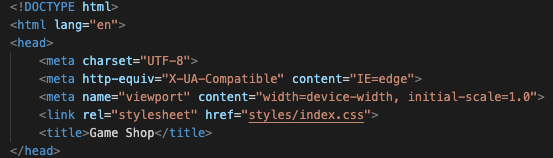
\includegraphics[scale=0.5]{head}
\end{center}

\subsection{Główne menu}

\begin{center}
	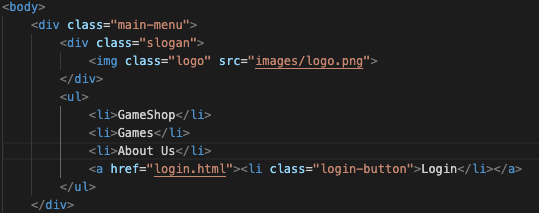
\includegraphics[scale=0.5]{menu}
\end{center}

\subsection{Wyszukanie gier}

\begin{center}
	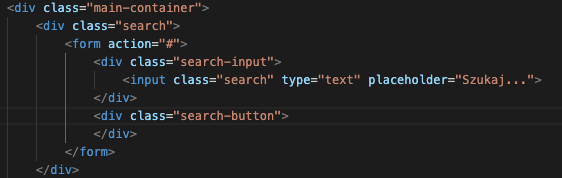
\includegraphics[scale=0.5]{search}
\end{center}

\subsection{Lista gier}

\begin{center}
	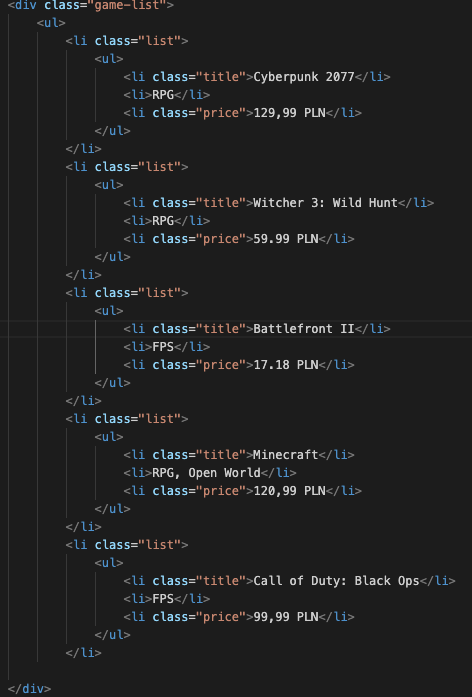
\includegraphics[scale=0.5]{games}
\end{center}

\subsection{Stopka}

\begin{center}
	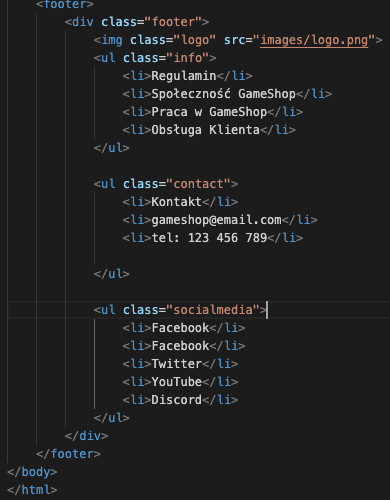
\includegraphics[scale=0.5]{footer}
\end{center}

\section{Struktura podstorny logowania}

\subsection{Formularz logowania}
\quad W strukturze podstrony z logowaniem lista z grami zamienia się na formularz logowania.

\begin{center}
	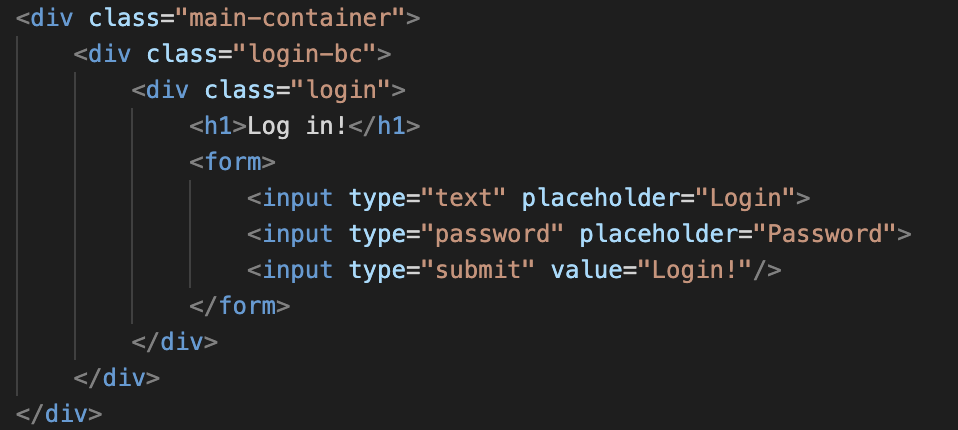
\includegraphics[scale=0.5]{login}
\end{center}

\section{Stylizacja strony}

\subsection{Style strony głównej}

\begin{center}
	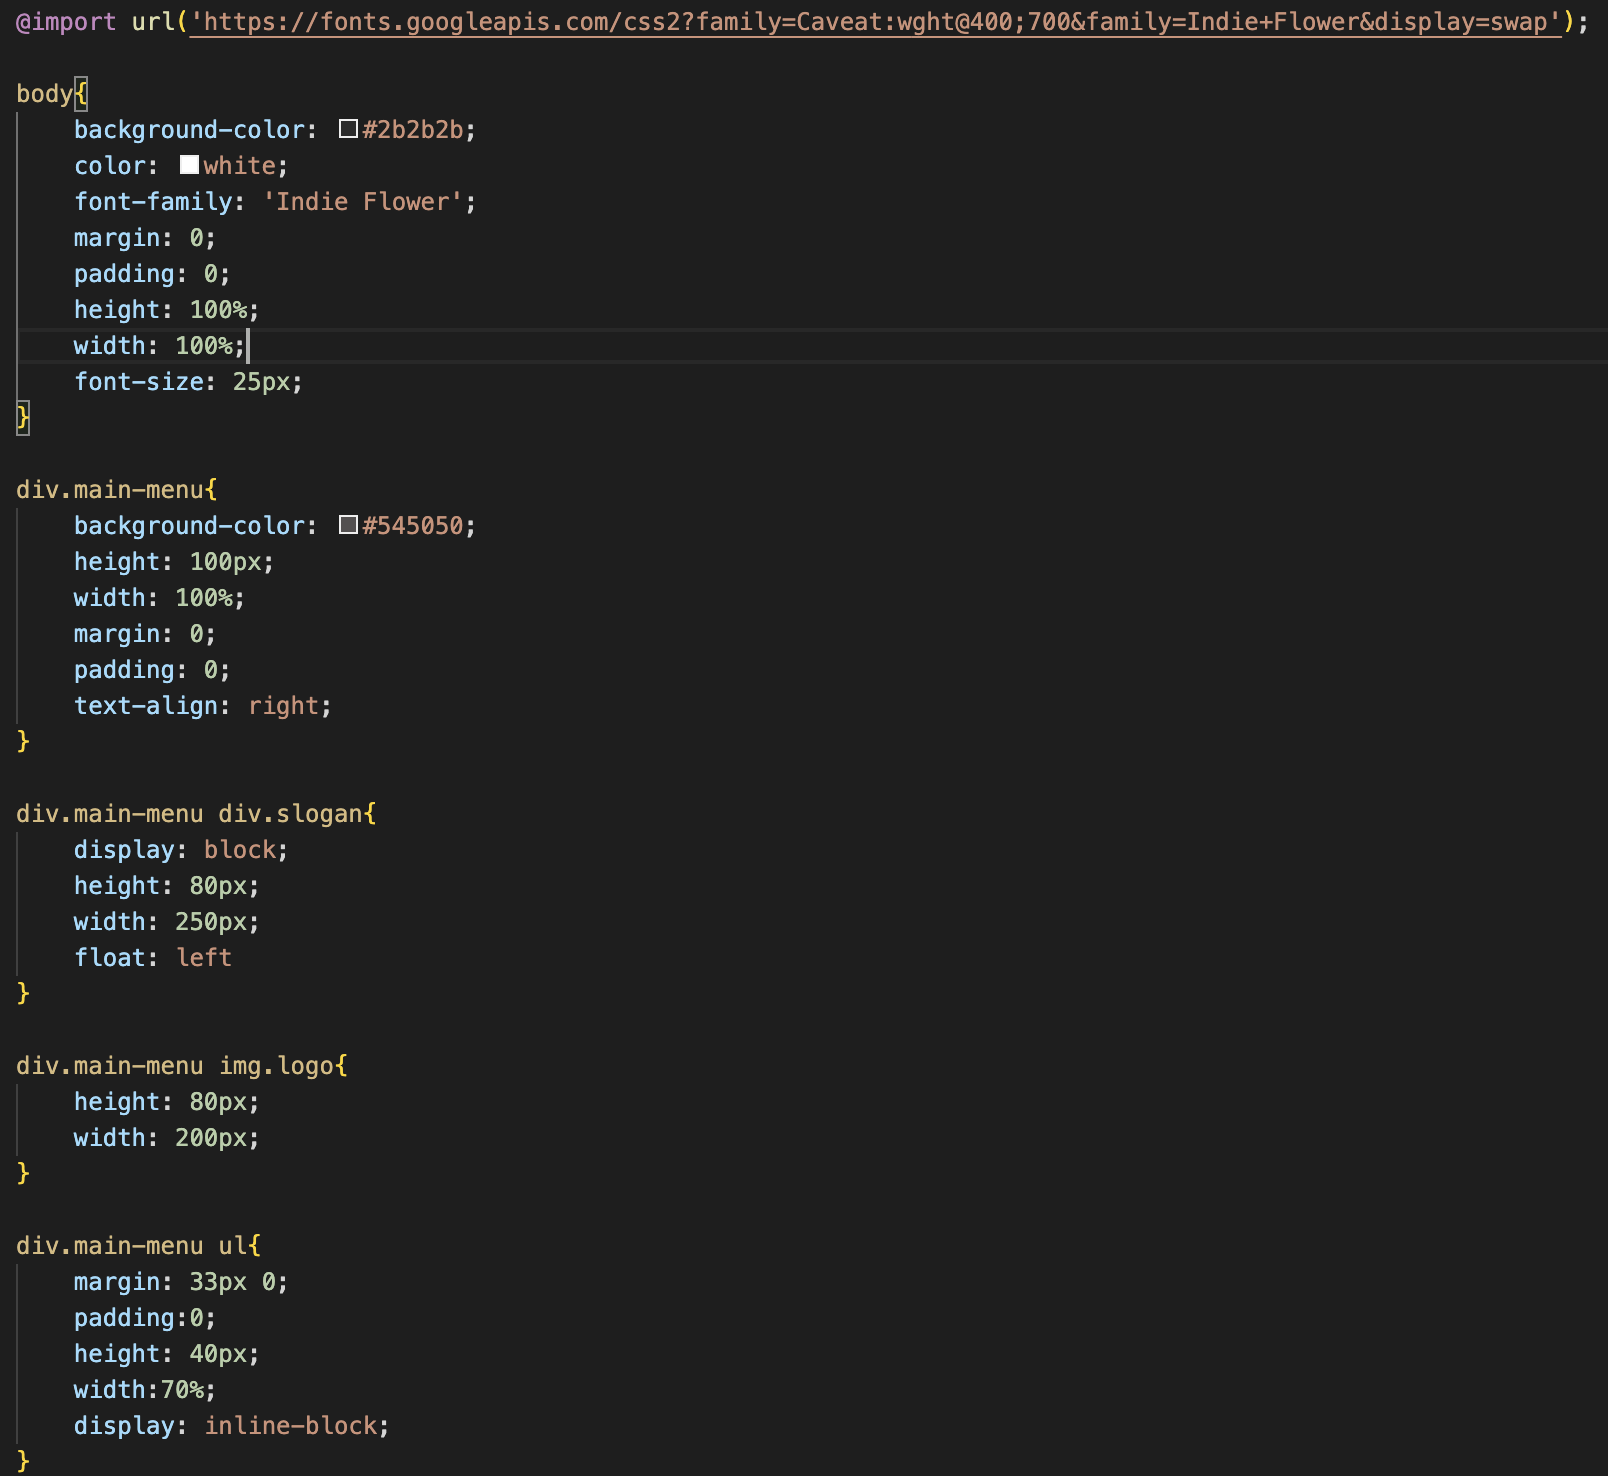
\includegraphics[scale=0.6]{style1}
\end{center}

\begin{center}
	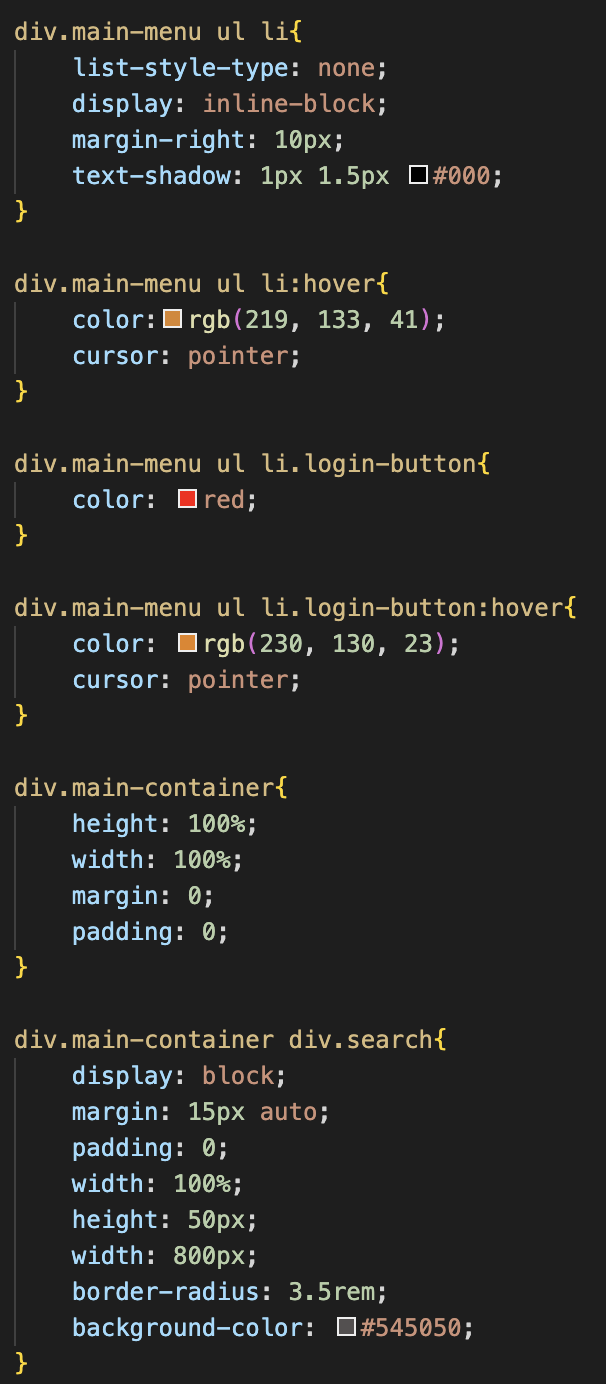
\includegraphics[scale=0.6]{style2}
\end{center}

\begin{center}
	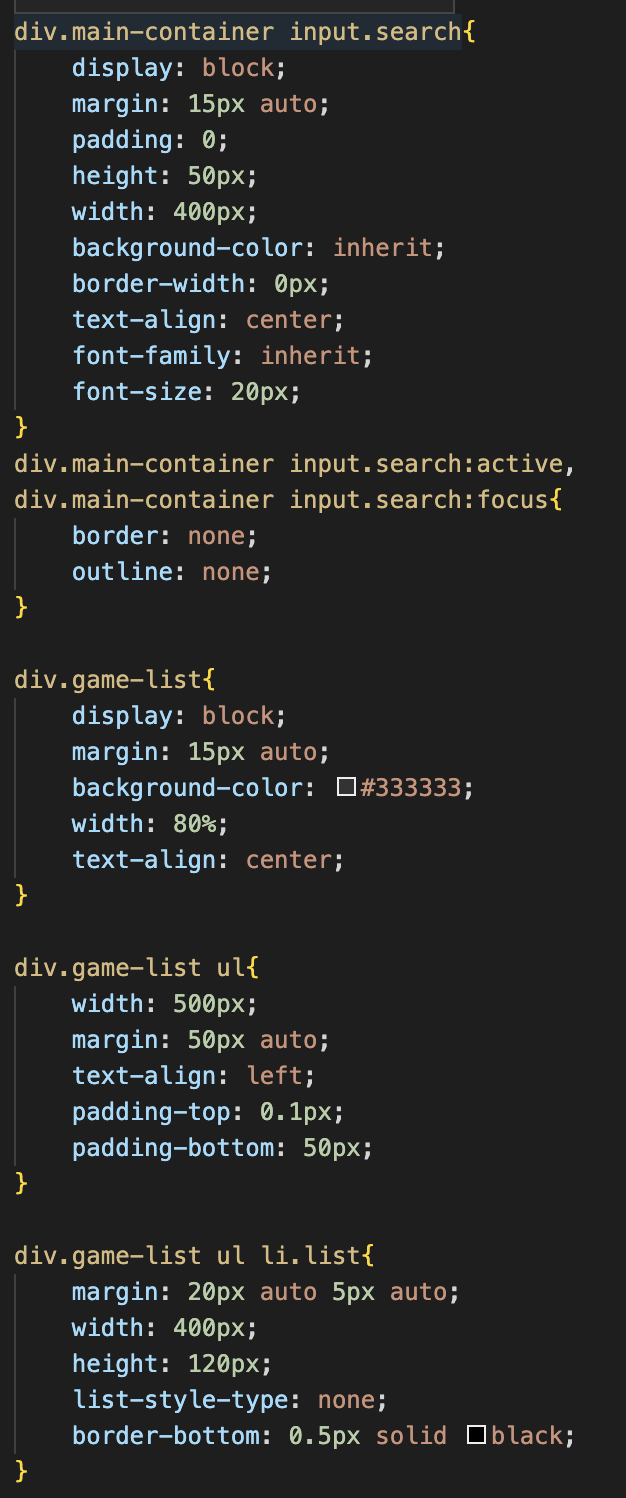
\includegraphics[scale=0.6]{style3}
\end{center}

\begin{center}
	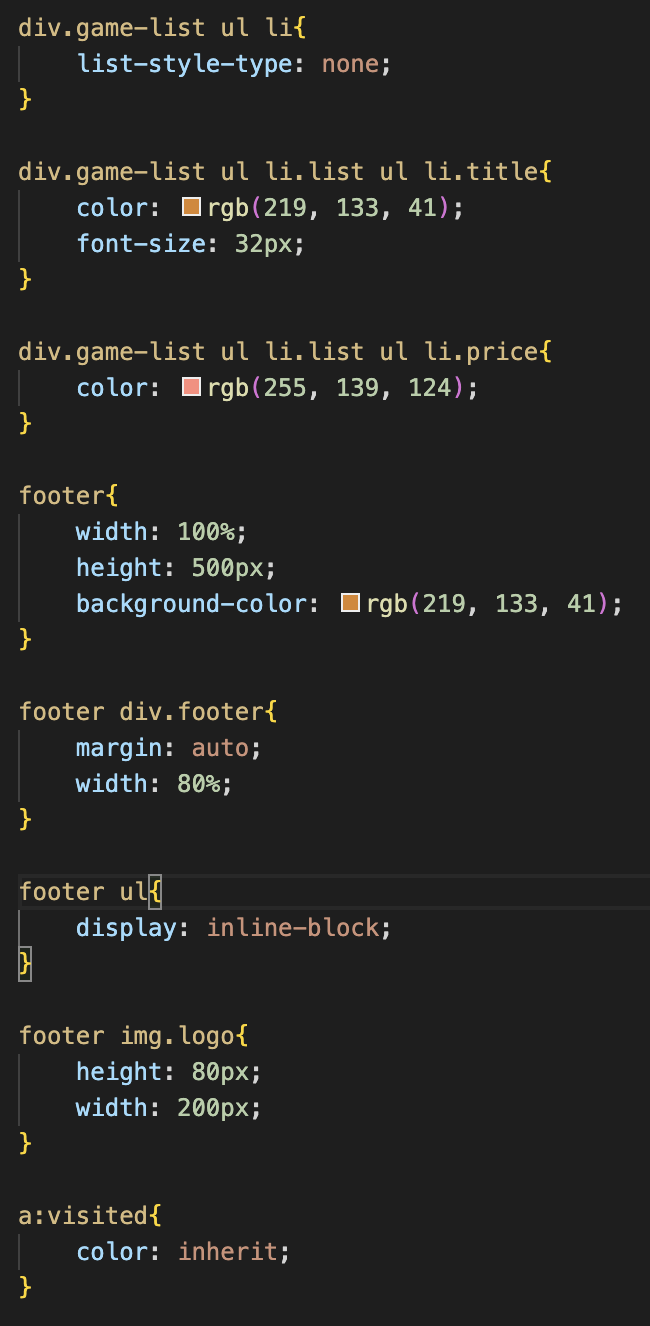
\includegraphics[scale=0.6]{style4}
\end{center}

\subsection{Style strony logowania}

\begin{center}
	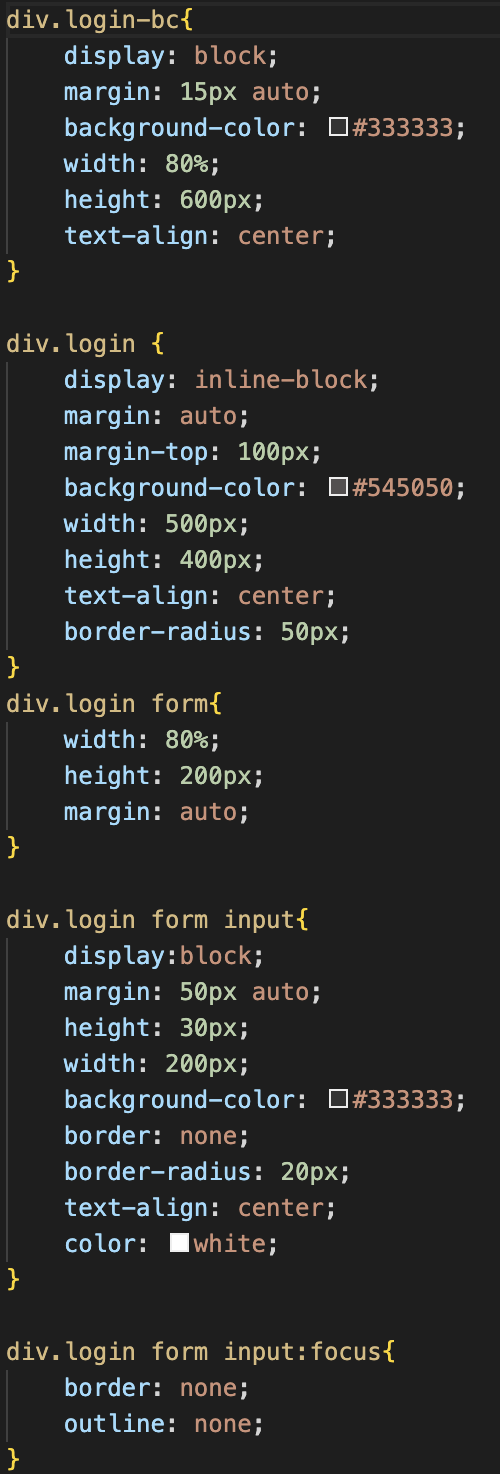
\includegraphics[scale=0.6]{style5}
\end{center}

\begin{center}
	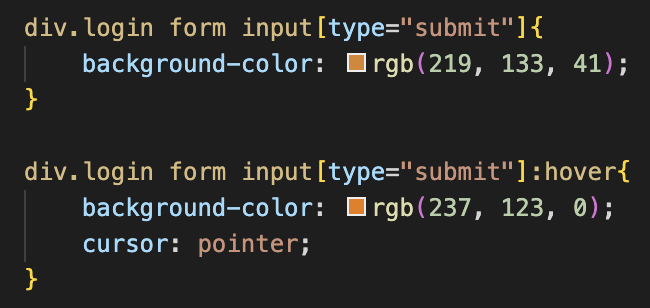
\includegraphics[scale=0.6]{style6}
\end{center}

\section{Opis techniczny projektu}
\begin{itemize}
\item Języki: HTML, CSS
\item Środowiska programistyczne: Visual Studio Code
\item Wersja VSC: 1.74.3 (Universal)
\end{itemize}


\end{document}